\documentclass{article}
\usepackage{graphicx} % Required for inserting images
\graphicspath{{img/}}
\usepackage{tikz}
\usepackage{circuitikz}
\usepackage{pgfplots}
\usepackage[spanish]{babel}
\usepackage{fancyhdr} 
\usepackage[bottom, norule]{footmisc}
\usepackage{multicol}    
\usepackage{sectsty}    
\usepackage{multicol}
\usepackage{amsmath}
\usepackage{hyperref}
\usepackage{listings}
\usepackage[table,dvipsnames]{xcolor}
\usepackage{listings}
\usepackage{accsupp}
\usepackage{float}
\usepackage{adjustbox}
\newcommand{\noncopynumber}[1]{
    \BeginAccSupp{method=escape,ActualText={}}
    #1
    \EndAccSupp{}
}
    \lstset{
    language=Python,
    backgroundcolor=\color{white},
    basicstyle=\ttfamily\footnotesize,
    keywordstyle=\color{blue},
    commentstyle=\color{green},
    stringstyle=\color{red},
    numbers=left,
    numberstyle=\tiny\color{gray},
    stepnumber=1,
    numbersep=10pt,
    frame=single,
    tabsize=4,
    captionpos=b,
    breaklines=true,
    breakatwhitespace=false,
    showspaces=false,
    showstringspaces=false,
    showtabs=false,
    morekeywords={np, plt} 
}

\title{Laboratorio 1}
\date{Octubre 2025}
\pgfplotsset{width=6cm}
\begin{document}
\fancyfoot[C]{}          
\fancyhead{}    
\begin{tikzpicture}[remember picture, overlay]
    \node[anchor=north west, xshift=2.6cm, yshift=-0.5cm] at (current page.north west) 
    {
\includegraphics[width=3.5cm]{img/marcaderecha.png}};
    \node[anchor=north east, xshift=-2.6cm, yshift=-1cm] at (current page.north east) 
    {
\includegraphics[width=4cm]{img/logo-cfm.png}}; 
\end{tikzpicture}

\begin{center}
\large Laboratorio 1 \\
\vspace{0.3cm}
{\scshape\Huge  Constante elástica de un resorte y Aceleración de gravedad \par}
\vspace{0.5cm}
\vspace{1.5cm}
{\large Autor: Bruno Bustos}
\vspace{0.3cm}
\large 
\\ 
\ttfamily{Universidad de Concepción, Facultad de Ciencias Físicas y Matemáticas.}
\end{center}
\vspace{1cm}

\begin{abstract}

    El objetivo de este informe es determinar la constante elástica de un resorte y la aceleración
    de gravedad mediante la medición experimental de la elongación de un resorte al colgarle diferentes
    masas y dejando caer un carrito a una distancia conocida, peso conocido y midiendo el tiempo que
    tarda en caer, respectivamente.

\end{abstract}

\begin{multicols}{2}

\section*{Introducción}

En esta Tarea se aborda la determinación experimental de
dos constantes físicas fundamentales: La aceleración de gravedad $g$
y la constante elástica de un resorte $k$.\\
La aceleración de gravedad es un parámetro fundamental que describe la
fuerza con la que la Tierra atrae a los objetos hacia su centro, mientras
que la constante elástica de un resorte caracteriza la rigidez de un resorte
y su relación  con la fuerza aplicada según la Ley de Hooke.\\
A través de experimentos prácticos, se buscará medir estas constantes de
manera directa, evaluando los posibles errores y comparando los resultados
experimentales con los valores teóricos.

\section*{Modelo Teórico}

    \subsection*{Aceleración de gravedad}

        La aceleración de gravedad $g$ se puede determinar mediante la medición del tiempo $t$ que tarda 
        un objeto en caer, en nuestro caso un carrito con ruedas que desprecian el roce, variando angulos
        de inclinación $\theta$ y conociendo la distancia $d$ recorrida. La relación entre estas variables
        está dada por la siguiente ecuación \ref{1} que sera  :

            \begin{equation}
                d = d_0 + tv_0 + \frac{1}{2} a t^2
            \end{equation}

        Donde:

            \begin{itemize}
                \item $d$ es la posición final (en metros, [m]).
                \item $d_0$ es la posición inicial (en metros, [m]).
                \item $v_0$ es la velocidad inicial (en metros por segundo, [m/s]).
                \item $a$ es la aceleración del objeto (en metros por segundo al cuadrado, [m/s²]).
                \item $t$ es el tiempo de caída (en segundos, [s]).
            \end{itemize}

        Pero podemos simplificar la ecuación ya que el carrito parte del reposo y la posición inicial 
        es cero, quedando de la siguiente forma:
            
            \begin{equation}
                d = \frac{1}{2} a t^2
            \end{equation}

        En el caso de un plano inclinado, la aceleración $a$ está relacionada con la aceleración de 
        gravedad $g$ y el ángulo de inclinación $\theta$ mediante la siguiente relación \ref{1}:

            \begin{equation}
                a = g \sin(\theta)
            \end{equation}

    \subsection*{Constante elástica de un resorte}

        La constante elástica de un resorte $k$ se define como la relación entre la fuerza $F$ aplicada al
        resorte y la elongación $\Delta x$ que experimenta, de acuerdo con la Ley de Hooke \ref{1}:

            \begin{equation}
                F = k \Delta x
            \end{equation}

        Donde:
            \begin{itemize}
                \item $F$ es la fuerza aplicada (en Newtons, N).
                \item $k$ es la constante elástica del resorte (en Newtons por metro, N/m).
                \item $\Delta x$ es la elongación del resorte (en metros, m).
            \end{itemize}
        Tambien tendremos que definir la segunda ley de Newton \ref{1}:

            \begin{equation}
                F = m \cdot a
            \end{equation}

        Donde:
            \begin{itemize}
                \item $F$ es la fuerza neta aplicada al objeto (en Newtons, N).
                \item $m$ es la masa del objeto (en kilogramos, kg).
                \item $a$ es la aceleración del objeto (en metros por segundo al cuadrado, m/s²).
            \end{itemize}

\section*{Procedimiento}

\subsection*{Determinación de la aceleración de gravedad}

    Se coloca la rampa inclinada en un ángulo conocido $\theta$. Se mide una distancia $d$ desde
    donde comienza el carrito hasta el punto donde se detiene. Se suelta el carrito y se registra
    el tiempo $t$ que tarda en recorrer la distancia $d$. Este proceso se repite para diferentes
    ángulos de inclinación. Se varía el ángulo 7 veces y para cada ángulo se registran 10 tiempos,
    se tomara el promedio de los tiempos para cada ángulo.
    \\ Tendremos una tabla con los ángulos y los tiempos promedios correspondientes:
    \begin{figure}[H]
    \begin{center}
        \begin{tabular}{|c|c|}
            \hline
            $\theta [Rad] \pm 0.009$ & $\bar{t} \pm 0.005 [s]$ \\
            \hline
            0.0698132 & 1.48 \\
            0.10472 & 1.15 \\
            0.139626 & 0.78 \\
            0.174533 & 0.84 \\
            0.20944 & 0.81 \\
            0.261799 & 0.62 \\
            0.314159 & 0.63 \\
            \hline
        \end{tabular}
    \end{center}
    \caption{Tabla de ángulos y tiempos promedios}
    \end{figure}
    Consideraremos un error instrumental en la medición del ángulo utilizando un transformador 
    de: 
        
        \begin{equation}
            \Delta \theta = 0.009 [Rad]
        \end{equation}
    
    Y un error en la medición del tiempo utilizando un cronómetro de:
        \begin{equation}
            \Delta t = 0.005 [s]
        \end{equation}

    Para determinar la aceleración de gravedad $g$, utilizaremos la relación entre la distancia recorrida
    por el carrito y el tiempo que tarda en recorrerla y la relación con la aceleración. La aceleración
    del carrito se puede calcular utilizando la siguiente ecuación del movimiento uniformemente acelerado:

    \begin{equation}
        d = \frac{1}{2} a t^2
    \end{equation}

    Despejando $a$, obtenemos:

    \begin{equation}
        a = \frac{2d}{t^2}
    \end{equation}
    Luego, utilizando la relación entre la aceleración $a$ y la aceleración de gravedad $g$ en un plano
    inclinado, tenemos:

    \begin{equation}
        a = g \sin(\theta)
    \end{equation}

    Despejando $g$, obtenemos:
    \begin{equation}
        g = \frac{a}{\sin(\theta)} = \frac{2d}{t^2 \sin(\theta)}
    \end{equation}

    Como necesitamos un ajuste lineal para determinar $g$, podemos reorganizar la ecuación anterior para obtener una
    relación lineal entre $t$ y $1/\sqrt{\sin(\theta)}$:

    \begin{equation}
        t = \sqrt{\frac{2d}{g}} \cdot \frac{1}{\sqrt{\sin(\theta)}}
    \end{equation}

    Lo que será un grafico lineal cuya pendiente nos permitirá calcular la aceleración de gravedad $g$.

    \begin{figure}[H]
        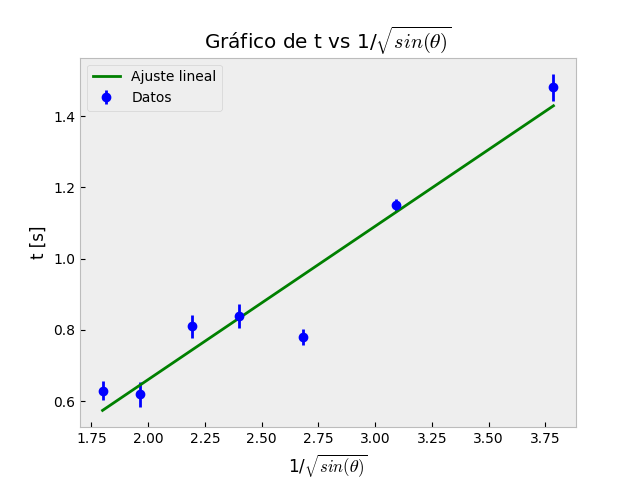
\includegraphics[width=\linewidth]{graf_gravedad.png}
    \caption{Gráfico de $t$ vs $\frac{1}{\sqrt{sin(\theta)}}$}
    \label{fig:plano_inclinado}
    \end{figure}

    Notamos que el valor obtenido para la aceleración de gravedad $g$ a partir del ajuste lineal es:

    \begin{equation}
        g = 10.281 \, [m/s^2]
    \end{equation}

    Ahora encontraremos el error asociado a $t$ que estara dado por la desviación estándar del promedio de los tiempos medidos
    para cada ángulo, y el error asociado a $\sin(\theta)$ que se puede calcular utilizando la fórmula de propagación de errores
    para funciones compuestas, primero calcularemos $\delta t$:

    \begin{equation}
        \delta t = \dfrac{\sigma_t}{\sqrt{N}}
    \end{equation}

    Conociendo que $\sigma_t$ es la desviación estándar de los tiempos medidos para cada ángulo y $N$ es el número de mediciones 
    (70 en este caso):

    \begin{equation}
        \sigma_t = \sqrt{\dfrac{\sum (t_i - \bar{t})^2}{N}}
    \end{equation}

    Donde $t_i$ son los tiempos individuales medidos y $\bar{t} = 0.90143 \, [s]$ es el tiempo promedio de $N = 70$ mediciones.

    Calculando $\sigma_t$ y luego $\delta t$, obtenemos:
    
    \begin{equation}
        \sigma_t = 0.2869 \, [s]
    \end{equation}

    \begin{equation}
        \delta t = 0.1084 \, [s]
    \end{equation}

    Y el error asociado a $\theta$ será solo $\delta \theta = 0.009 \, [Rad]$.

    Ahora calcularemos el error asociado a la aceleración de gravedad $g$. Utilizando la fórmula de propagación de errores
    para una función de variables dependientes, tenemos que:

    \begin{equation}
        \delta g = \left|\dfrac{\partial g}{\partial t}\right| \delta t + \left|\dfrac{\partial g}{\partial \theta}\right| \delta \theta
    \end{equation}

    Donde:
    \begin{itemize}
        \item $\delta g$ es el error en la aceleración de gravedad.
        \item $\delta t$ es el error en el tiempo medido.
        \item $\delta \theta$ es el error del ángulo de inclinación.
    \end{itemize}

    Calculando las derivadas parciales y sustituyendo los valores, obtenemos:

    \begin{equation}
        \delta g = \dfrac{4d}{t^3 \sin(\theta)} \delta t + \dfrac{2d \cos(\theta)}{t^2 \sin^2(\theta)} \delta \theta
    \end{equation}

    sustituyendo los valores promedio de $t$ y $\bar{\theta} = 0.18201 \, [Rad]$, obtenemos:

    \begin{equation}
        \delta g = 3.7 \, [m/s^2]
    \end{equation}

    Por lo que el valor final de la aceleración de gravedad con su error asociado es:

    \begin{equation}
        g = 10.3 \pm 3.7 \, [m/s^2]
    \end{equation}

\subsection*{Determinación de la constante elástica de un resorte}

    Primero se cuelga el resorte del soporte y se mide su longitud inicial sin ninguna masa colgada.
    Luego, se cuelgan diferentes masas conocidas al resorte y se mide la elongación del resorte 
    para cada masa. Se repite este proceso para 14 masas diferentes, registrando 14 elongaciones 
    distintas.
    \\ Tendremos una tabla con las masas y las elongaciones correspondientes:
    \begin{figure}[H]
    \begin{center}
        \begin{tabular}{|c|c|}
            \hline
            $ m [kg]$ & $ d [m]$ \\
            \hline
            0.026 & 0.3 \\
            0.041 & 0.4 \\
            0.048 & 0.9 \\
            0.090 & 2.3 \\
            0.105 & 3.0 \\
            0.187 & 5.3 \\
            0.250 & 7.5 \\
            0.339 & 10.2 \\
            0.417 & 12.8 \\
            0.410 & 15.4 \\
            0.750 & 23.6 \\
            0.798 & 24.9 \\
            0.999 & 31.1 \\
            1.123 & 35.5 \\
            \hline
        \end{tabular}
    \end{center}
    \caption{Tabla de masas y elongaciones}
    \end{figure}
    Consideraremos un error instrumental en la medición de la elongación utilizando una regla
    de:
    
    \begin{equation}
        \Delta d \approx 0 [m]
    \end{equation}

    Ya que la regla tiene alta precisión y un error en la medición de la masa utilizando una balanza de:

    \begin{equation}
        \Delta m \approx 0 [kg]
    \end{equation}

    Para calcular la constante elástica del resorte $k$, utilizaremos la segunda Ley de Newton
        y la Ley de Hooke. La fuerza aplicada al resorte es igual al peso de la masa colgada ya que
        está en equilibrio, es decir, $F = m \cdot g$, donde $g$ es la aceleración de gravedad 
        (aproximadamente $10.3 \pm 3.7\, [m/s^2]$). 

        \begin{equation}
            m \cdot g = k \cdot \Delta d
        \end{equation}

        Despejando $k$, obtenemos:
        \begin{equation}
            k = \frac{m \cdot g}{\Delta d}
        \end{equation}

        Como consideramos nuestro punto de origen en la posición del resorte sin masa colgada,
        la elongación $\Delta d$ es simplemente la longitud medida del resorte con la masa colgada, ademas
        podemos notar que existe una relación lineal entre la masa colgada y la elongación del resorte,
        por lo que podemos graficar masa vs elongación y obtener la pendiente de la recta, que sera igual
        a:

        \begin{equation}
            d = \dfrac{g}{m} \cdot k
        \end{equation}

        Lo que será un grafico lineal cuya pendiente nos permitirá calcular la constante elástica del resorte 
        $k$.

        \begin{figure}[H]
            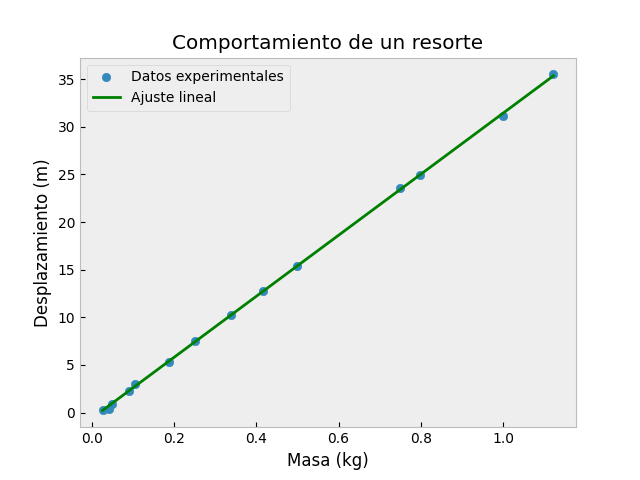
\includegraphics[width=\linewidth]{Cons_elast.png}
        \caption{Gráfico de masa vs elongación del resorte}
        \label{fig:resorte}
        \end{figure}

        Analizando el gráfico de la figura \ref{fig:resorte}, podemos observar que los datos experimentales
        se ajustan bastante bien a una línea recta, lo que confirma la relación lineal entre la masa colgada y la elongación del resorte.
        Utilizando un ajuste lineal a los datos, se obtiene una pendiente que nos permite calcular la constante elástica del resorte $k$.
        El valor obtenido para la constante elástica del resorte es:

        \begin{equation}
            k = 32.02 \, [N/m]
        \end{equation}

        Ahora encontraremos el error asociado a la constante elástica $k$. Utilizando la fórmula de propagación de errores
        para una función de variables dependientes, tenemos que:
        \begin{equation}
            \delta k = \left|\dfrac{\partial k}{\partial m}\right| \delta m + \left|\dfrac{\partial k}{\partial d}\right| \delta d + \left|\dfrac{\partial k}{\partial g}\right| \delta g
        \end{equation}
        Donde:
        \begin{itemize}
            \item $\delta k$ es el error en la constante elástica del resorte.
            \item $\delta m$ es el error en la masa colgada.
            \item $\delta d$ es el error en la elongación del resorte.
            \item $\delta g$ es el error en la aceleración de gravedad.
        \end{itemize}

        Pero como $\delta m \approx 0$ y $\delta d \approx 0$, la ecuación se simplifica a:
        
        \begin{equation}
            \delta k = \left|\dfrac{\partial k}{\partial g}\right| \delta g
        \end{equation}

        Calculando la derivada parcial y sustituyendo los valores, obtenemos:

        \begin{equation}
            \delta k = \dfrac{m}{d} \delta g
        \end{equation}

        Sustituyendo los valores promedio de $m = 0.40511$, $d = 12.37143$ y el $\delta g$ obtenemos:

        \begin{equation}
            \delta k = 0.1 \, [N/m]
        \end{equation}

        Por lo que el valor final de la constante elástica del resorte con su error asociado es:

        \begin{equation}
            k = 32.0 \pm 0.1 \, [N/m]
        \end{equation}

\subsection*{Resultados finales}

    \begin{itemize}
        \item Aceleración de gravedad: $g = 10.3 \pm 3.7 \, [m/s^2]$
        \item Constante elástica del resorte: $k = 32.0 \pm 0.1 \, [N/m]$
    \end{itemize}

\section*{Discusión}

    En este informe se ha logrado determinar experimentalmente dos constantes físicas fundamentales:
    la aceleración de gravedad $g$ y la constante elástica de un resorte $k$ mediante métodos prácticos.
    Es claro que existen diversas fuentes de error que pueden haber afectado la precisión de los resultados
    obtenidos. En el caso de $g$, los errores en la medición del tiempo y el ángulo de inclinación pueden
    haber contribuido significativamente a la incertidumbre final. Además, la suposición de que el carrito
    no experimenta rozamiento puede no ser completamente válida, lo que podría haber afectado la 
    aceleración calculada.\\
    En cuanto a la constante elástica $k$, aunque el ajuste lineal mostró una buena correlación entre
    la masa colgada y la elongación del resorte, es posible que factores como la precisión en la medición
    de la masa y la elongación hayan introducido errores adicionales. Además, al utilizar el valor de $g$
    obtenido previamente, cualquier error en este valor se propaga directamente a la incertidumbre en $k$.
    \\ A pesar de estas limitaciones, los resultados obtenidos son razonables y están dentro de un rango
    aceptable considerando las condiciones experimentales. Para mejorar la precisión en futuros 
    experimentos se podrían implementar métodos más sofisticados de medición, como el uso de sensores
    electrónicos para el tiempo y la elongación, así como considerar el efecto del rozamiento en el 
    análisis de datos o mejorar el tipo de material utilizado en el resorte para minimizar posibles 
    deformaciones.

\section*{Conclusión}

    En conclusión, este informe ha demostrado la viabilidad de determinar experimentalmente la aceleración
    de gravedad $g$ y la constante elástica de un resorte $k$ mediante métodos prácticos. A pesar de las
    limitaciones y fuentes de error identificadas, los resultados obtenidos son consistentes con los
    valores esperados y proporcionan una base sólida de lo que es posible lograr en un entorno de 
    laboratorio. Los métodos utilizados, aunque simples, han permitido una comprensión más profunda de 
    los conceptos involucrados como la interpretación de datos experimentales y la propagación de errores.
    Estos resultados resaltan la importancia de la precisión en las mediciones y el análisis cuidadoso
    de los datos en experimentos físicos. Futuras investigaciones podrían centrarse en mejorar la
    precisión de las mediciones y explorar otros métodos para determinar estas constantes físicas,
    contribuyendo así al avance del conocimiento en el campo de la física experimental.

\section*{Códigos utilizados}

\begin{figure}[H]
        \begin{center}
        \begin{adjustbox}{max width=1.0\linewidth}
        \begin{lstlisting}
import numpy as np
import matplotlib.pyplot as plt
plt.style.use("bmh")

datos4 = np.genfromtxt("Tareas\Tarea02\Compl\datos_resorte.txt")

x = datos4[:,0]
y = datos4[:,1]

coef_polinomios = np.polyfit(x, y, 1)
#Ajustar un polinomio de grado n a los datos (x, y)

polinomio = np.poly1d(coef_polinomios)

u = np.linspace(min(x), max(x), 100)

v = polinomio(u)
#Evaluar el polinomio en los puntos generados

print("Constante elastica k =", coef_polinomios[0], "N/m")

plt.scatter(x, y)
plt.plot(u, v, "r-", color='green', linewidth=2)

plt.legend(["Datos experimentales", "Ajuste lineal"])
plt.xlabel("Masa (kg)")
plt.ylabel("Desplazamiento (m)")
plt.title("Comportamiento de un resorte")
plt.grid()
plt.show()
        \end{lstlisting}
        \end{adjustbox}
        \end{center}
    \caption{Códigos en python usados para graficar los datos}
    \label{fig:resorte1}
    \end{figure}

    \begin{figure}[H]
        \begin{center}
        \begin{adjustbox}{max width=1.0\linewidth}
        \begin{lstlisting}
import numpy as np
import matplotlib.pyplot as plt
plt.style.use("bmh")

datos5 = np.genfromtxt("Tareas\Tarea02\Compl\datos_car.txt")

theta = datos5[:,0]
t = datos5[:,1]
err = datos5[:,2]

x = 1 / np.sqrt(np.sin(theta))
y = t              

coef_polinomios = np.polyfit(x, y, 1)

polinomio = np.poly1d(coef_polinomios)

u = np.linspace(min(x), max(x), 100)

v = polinomio(u)

L = 0.95

m = coef_polinomios[0]

g = 2*L/m**2

delta_g = 2*L*err**2/m**4

plt.errorbar(x, y, yerr=err, fmt='o', color='blue', label='Datos')
plt.plot(u, v, "r-", color="green", linewidth=2, label="Ajuste lineal")
plt.xlabel("1/$\sqrt{sin(theta)}$")
plt.ylabel("t [s]")
plt.title("Grafico de t vs 1/$\sqrt{sin(theta)}$")
plt.legend()
plt.grid()
plt.show()

print(f"Pendiente de la recta: m = {m:.3f}")
print(f"Gravedad calculada: g = {g:.3f} m/s**2")
        \end{lstlisting}
        \end{adjustbox}
        \end{center}
    \caption{Códigos en python usados para graficar los datos}
    \label{fig:car1}
    \end{figure}

\section*{Referencias}
    \begin{enumerate}
    
        \item \label{1} Resnick, R., Halliday, D., \& Krane, K. (1988). 
        \textit{Physics, Vol. 1} (4th ed.). John Wiley \& Sons. 
    
    \end{enumerate}
\end{multicols}
\end{document}